% Options for packages loaded elsewhere
\PassOptionsToPackage{unicode}{hyperref}
\PassOptionsToPackage{hyphens}{url}
%
\documentclass[
]{article}
\usepackage{lmodern}
\usepackage{amssymb,amsmath}
\usepackage{ifxetex,ifluatex}
\ifnum 0\ifxetex 1\fi\ifluatex 1\fi=0 % if pdftex
  \usepackage[T1]{fontenc}
  \usepackage[utf8]{inputenc}
  \usepackage{textcomp} % provide euro and other symbols
\else % if luatex or xetex
  \usepackage{unicode-math}
  \defaultfontfeatures{Scale=MatchLowercase}
  \defaultfontfeatures[\rmfamily]{Ligatures=TeX,Scale=1}
\fi
% Use upquote if available, for straight quotes in verbatim environments
\IfFileExists{upquote.sty}{\usepackage{upquote}}{}
\IfFileExists{microtype.sty}{% use microtype if available
  \usepackage[]{microtype}
  \UseMicrotypeSet[protrusion]{basicmath} % disable protrusion for tt fonts
}{}
\makeatletter
\@ifundefined{KOMAClassName}{% if non-KOMA class
  \IfFileExists{parskip.sty}{%
    \usepackage{parskip}
  }{% else
    \setlength{\parindent}{0pt}
    \setlength{\parskip}{6pt plus 2pt minus 1pt}}
}{% if KOMA class
  \KOMAoptions{parskip=half}}
\makeatother
\usepackage{xcolor}
\IfFileExists{xurl.sty}{\usepackage{xurl}}{} % add URL line breaks if available
\IfFileExists{bookmark.sty}{\usepackage{bookmark}}{\usepackage{hyperref}}
\hypersetup{
  pdftitle={lista 1 Econometria},
  pdfauthor={Miguel Sallum},
  hidelinks,
  pdfcreator={LaTeX via pandoc}}
\urlstyle{same} % disable monospaced font for URLs
\usepackage[margin=1in]{geometry}
\usepackage{color}
\usepackage{fancyvrb}
\newcommand{\VerbBar}{|}
\newcommand{\VERB}{\Verb[commandchars=\\\{\}]}
\DefineVerbatimEnvironment{Highlighting}{Verbatim}{commandchars=\\\{\}}
% Add ',fontsize=\small' for more characters per line
\usepackage{framed}
\definecolor{shadecolor}{RGB}{248,248,248}
\newenvironment{Shaded}{\begin{snugshade}}{\end{snugshade}}
\newcommand{\AlertTok}[1]{\textcolor[rgb]{0.94,0.16,0.16}{#1}}
\newcommand{\AnnotationTok}[1]{\textcolor[rgb]{0.56,0.35,0.01}{\textbf{\textit{#1}}}}
\newcommand{\AttributeTok}[1]{\textcolor[rgb]{0.77,0.63,0.00}{#1}}
\newcommand{\BaseNTok}[1]{\textcolor[rgb]{0.00,0.00,0.81}{#1}}
\newcommand{\BuiltInTok}[1]{#1}
\newcommand{\CharTok}[1]{\textcolor[rgb]{0.31,0.60,0.02}{#1}}
\newcommand{\CommentTok}[1]{\textcolor[rgb]{0.56,0.35,0.01}{\textit{#1}}}
\newcommand{\CommentVarTok}[1]{\textcolor[rgb]{0.56,0.35,0.01}{\textbf{\textit{#1}}}}
\newcommand{\ConstantTok}[1]{\textcolor[rgb]{0.00,0.00,0.00}{#1}}
\newcommand{\ControlFlowTok}[1]{\textcolor[rgb]{0.13,0.29,0.53}{\textbf{#1}}}
\newcommand{\DataTypeTok}[1]{\textcolor[rgb]{0.13,0.29,0.53}{#1}}
\newcommand{\DecValTok}[1]{\textcolor[rgb]{0.00,0.00,0.81}{#1}}
\newcommand{\DocumentationTok}[1]{\textcolor[rgb]{0.56,0.35,0.01}{\textbf{\textit{#1}}}}
\newcommand{\ErrorTok}[1]{\textcolor[rgb]{0.64,0.00,0.00}{\textbf{#1}}}
\newcommand{\ExtensionTok}[1]{#1}
\newcommand{\FloatTok}[1]{\textcolor[rgb]{0.00,0.00,0.81}{#1}}
\newcommand{\FunctionTok}[1]{\textcolor[rgb]{0.00,0.00,0.00}{#1}}
\newcommand{\ImportTok}[1]{#1}
\newcommand{\InformationTok}[1]{\textcolor[rgb]{0.56,0.35,0.01}{\textbf{\textit{#1}}}}
\newcommand{\KeywordTok}[1]{\textcolor[rgb]{0.13,0.29,0.53}{\textbf{#1}}}
\newcommand{\NormalTok}[1]{#1}
\newcommand{\OperatorTok}[1]{\textcolor[rgb]{0.81,0.36,0.00}{\textbf{#1}}}
\newcommand{\OtherTok}[1]{\textcolor[rgb]{0.56,0.35,0.01}{#1}}
\newcommand{\PreprocessorTok}[1]{\textcolor[rgb]{0.56,0.35,0.01}{\textit{#1}}}
\newcommand{\RegionMarkerTok}[1]{#1}
\newcommand{\SpecialCharTok}[1]{\textcolor[rgb]{0.00,0.00,0.00}{#1}}
\newcommand{\SpecialStringTok}[1]{\textcolor[rgb]{0.31,0.60,0.02}{#1}}
\newcommand{\StringTok}[1]{\textcolor[rgb]{0.31,0.60,0.02}{#1}}
\newcommand{\VariableTok}[1]{\textcolor[rgb]{0.00,0.00,0.00}{#1}}
\newcommand{\VerbatimStringTok}[1]{\textcolor[rgb]{0.31,0.60,0.02}{#1}}
\newcommand{\WarningTok}[1]{\textcolor[rgb]{0.56,0.35,0.01}{\textbf{\textit{#1}}}}
\usepackage{graphicx,grffile}
\makeatletter
\def\maxwidth{\ifdim\Gin@nat@width>\linewidth\linewidth\else\Gin@nat@width\fi}
\def\maxheight{\ifdim\Gin@nat@height>\textheight\textheight\else\Gin@nat@height\fi}
\makeatother
% Scale images if necessary, so that they will not overflow the page
% margins by default, and it is still possible to overwrite the defaults
% using explicit options in \includegraphics[width, height, ...]{}
\setkeys{Gin}{width=\maxwidth,height=\maxheight,keepaspectratio}
% Set default figure placement to htbp
\makeatletter
\def\fps@figure{htbp}
\makeatother
\setlength{\emergencystretch}{3em} % prevent overfull lines
\providecommand{\tightlist}{%
  \setlength{\itemsep}{0pt}\setlength{\parskip}{0pt}}
\setcounter{secnumdepth}{-\maxdimen} % remove section numbering
\usepackage[brazilian]{babel}
\usepackage[utf8]{inputenc}

\title{lista 1 Econometria}
\author{Miguel Sallum}
\date{24/05/2021}

\begin{document}
\maketitle

\hypertarget{questuxe3o-1}{%
\subsection{Questão 1}\label{questuxe3o-1}}

Com os dados da tabela abaixo, estime a regressão de Y em função de X2 e
X3 e faça os testes da regressão e de cada um dos parâmetros.

\begin{Shaded}
\begin{Highlighting}[]
\NormalTok{Y <-}\StringTok{ }\KeywordTok{c}\NormalTok{(}\DecValTok{800}\NormalTok{, }\DecValTok{1160}\NormalTok{, }\DecValTok{1580}\NormalTok{, }\DecValTok{2010}\NormalTok{, }\DecValTok{1890}\NormalTok{, }\DecValTok{2600}\NormalTok{, }\DecValTok{2070}\NormalTok{, }\DecValTok{1890}\NormalTok{, }\DecValTok{1830}\NormalTok{, }\DecValTok{1740}\NormalTok{, }\DecValTok{1380}\NormalTok{, }\DecValTok{1060}\NormalTok{)}

\NormalTok{X <-}\StringTok{ }\KeywordTok{tibble}\NormalTok{(}
\NormalTok{  X1 <-}\StringTok{ }\DecValTok{1}\NormalTok{,}
\NormalTok{  X2 <-}\StringTok{ }\KeywordTok{c}\NormalTok{(}\DecValTok{2}\NormalTok{, }\DecValTok{4}\NormalTok{, }\DecValTok{6}\NormalTok{, }\DecValTok{8}\NormalTok{, }\DecValTok{7}\NormalTok{, }\DecValTok{12}\NormalTok{, }\DecValTok{11}\NormalTok{, }\DecValTok{10}\NormalTok{, }\DecValTok{9}\NormalTok{, }\DecValTok{8}\NormalTok{, }\DecValTok{6}\NormalTok{, }\DecValTok{4}\NormalTok{),}
\NormalTok{  X3 <-}\StringTok{ }\KeywordTok{c}\NormalTok{(.}\DecValTok{8}\NormalTok{, }\FloatTok{.7}\NormalTok{, }\FloatTok{.5}\NormalTok{, }\FloatTok{.4}\NormalTok{, }\FloatTok{.2}\NormalTok{, }\FloatTok{.2}\NormalTok{, }\FloatTok{.8}\NormalTok{, }\FloatTok{.7}\NormalTok{, }\FloatTok{.6}\NormalTok{, }\FloatTok{.1}\NormalTok{, }\FloatTok{.5}\NormalTok{, }\FloatTok{.4}\NormalTok{)}
\NormalTok{)}
\end{Highlighting}
\end{Shaded}

O modelo a ser estimado é:

\[Y\ =\ \beta_1\ +\ \beta_2X_2\ +\ \beta_3X_3\ +\ v_t\]

A Calcule os parâmetros \(\beta_{1},\ \beta_{2},\ \beta_{3}\) desse
modelo. B Monte a matriz de resíduos deste modelo. Calcule a soma dos
quadrados dos resíduos utilizando método matricial. ´ C Calcule o
R\textsuperscript{2} deste modelo. D Monte a matriz de variância e
covariância deste modelo. ˆ E Verifique se os
\(\beta_{1},\ \beta_{2},\ \beta_{3}\) sao significantes ao nível de 5\%
de significância.

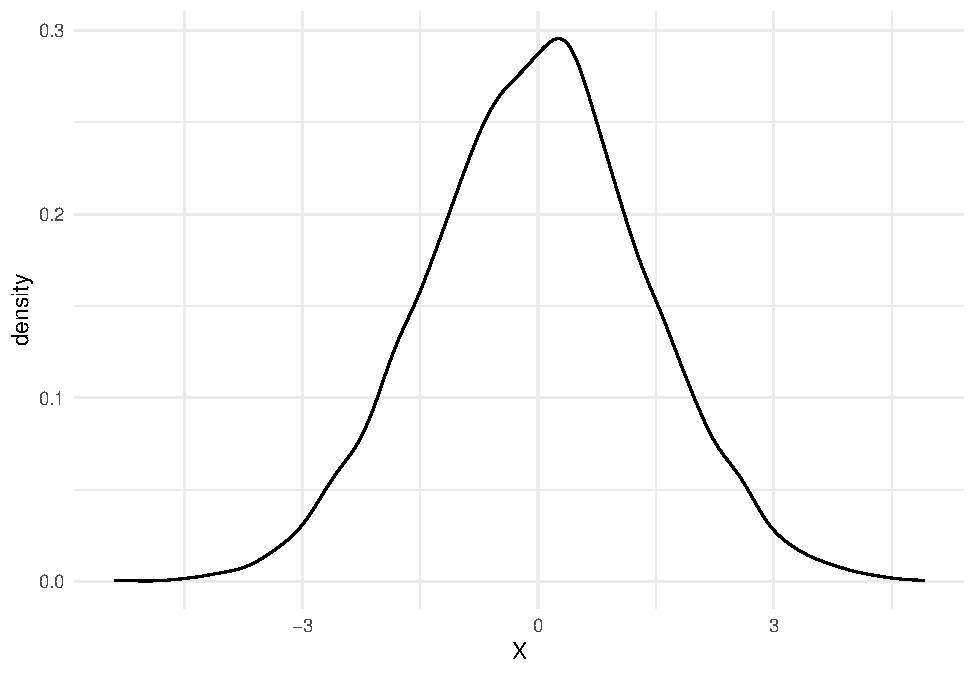
\includegraphics{lista_1_files/figure-latex/pressure-1.pdf}

\hypertarget{questuxe3o-2}{%
\subsection{Questão 2}\label{questuxe3o-2}}

A questão anterior adicionamos uma variável \emph{dummy}, que representa
a existência ou não de determinado atributo.

\begin{Shaded}
\begin{Highlighting}[]
\NormalTok{Xd <-}\StringTok{ }\NormalTok{X }\OperatorTok
\StringTok{  }\KeywordTok{mutate}\NormalTok{(}
    \DataTypeTok{D=} \KeywordTok{c}\NormalTok{(}\KeywordTok{rep}\NormalTok{(}\DecValTok{1}\NormalTok{, }\DecValTok{6}\NormalTok{), }\KeywordTok{rep}\NormalTok{(}\DecValTok{0}\NormalTok{, }\DecValTok{6}\NormalTok{))}
\NormalTok{  )}
\end{Highlighting}
\end{Shaded}

O modelo a ser estimado é:

\[Y\ =\ \beta_1\ +\ \beta_2X_2\ +\ \beta_3X_3\ +\ \beta_4D\ +\ v_t\]

A Calcule os parâmetros \(\beta_{1},\ \beta_{2},\ \beta_{3}\) desse
modelo. B Monte a matriz de resíduos deste modelo. Calcule a soma dos
quadrados dos resíduos utilizando método matricial. ´ C Calcule o
R\textsuperscript{2} deste modelo. D Monte a matriz de variância e
covariância robusta deste modelo. ˆ E Verifique se os
\(\beta_{1},\ \beta_{2},\ \beta_{3}\) sao significantes ao nível de 5\%
de significância.

\hypertarget{questuxe3o-3}{%
\subsection{Questão 3}\label{questuxe3o-3}}

Use os valores descritos na tabela abaixo para ilustrar que
\(E[Yi(0)] − E[Yi(1)] =E[Yi(0) − Yi(1)]\)

\begin{Shaded}
\begin{Highlighting}[]
\NormalTok{vilas <-}\StringTok{ }\KeywordTok{tibble}\NormalTok{(}
  \DataTypeTok{vila =} \DecValTok{1}\OperatorTok{:}\DecValTok{7}\NormalTok{,}
  \DataTypeTok{Y0 =} \KeywordTok{c}\NormalTok{(}\DecValTok{10}\NormalTok{, }\DecValTok{15}\NormalTok{, }\DecValTok{20}\NormalTok{, }\DecValTok{20}\NormalTok{, }\DecValTok{10}\NormalTok{, }\DecValTok{15}\NormalTok{, }\DecValTok{15}\NormalTok{),}
  \DataTypeTok{Y1 =} \KeywordTok{c}\NormalTok{(}\DecValTok{15}\NormalTok{, }\DecValTok{15}\NormalTok{, }\DecValTok{30}\NormalTok{, }\DecValTok{15}\NormalTok{, }\DecValTok{20}\NormalTok{, }\DecValTok{15}\NormalTok{, }\DecValTok{30}\NormalTok{),}
  \DataTypeTok{tau =}\NormalTok{ Y1}\OperatorTok{-}\StringTok{ }\NormalTok{Y0}
\NormalTok{)}
\end{Highlighting}
\end{Shaded}

\hypertarget{questuxe3o-4}{%
\subsection{Questão 4}\label{questuxe3o-4}}

Demonstre como chegar nessa igualdade:

\[\frac{1}{N_t}\sum_{i=1}^n( y_i | d_i=1)\ +\ \frac{1}{N_C}\sum_{i=1}^n( y_i | d_i=0)\ =\ E[Y^1]\ -\ E[Y^0]\]\newline \[+\ E[Y^0|D=1]\ -\ E[Y^0|D=0]\ +\ (1\ -\ \pi)(ATT\ -\ ATU) \]

\hypertarget{questuxe3o-5}{%
\subsection{Questão 5}\label{questuxe3o-5}}

Em que condições teremos a seguinte igualdade? Justifique

\[\frac{1}{N_t}\sum_{i=1}^n( y_i | d_i=1)\ +\ \frac{1}{N_C}\sum_{i=1}^n( y_i | d_i=0)\ =\ E[Y^1]\ -\ E[Y^0]\]

\hypertarget{questuxe3o-6}{%
\subsection{Questão 6}\label{questuxe3o-6}}

Suponha que um laboratório esteja testando um novo medicamento que tem
como objetivo prolongar a vida de pacientes com câncer. Para realizar o
estudo, os cientistas irão dividir sua amostra em dois grupos. Os
indíviduos pares são os indivíduos do grupo tratamento e que tomam o
medicamento, enquanto que os indivíduos ímpares pertencem ao grupo
controle e tomam um placebo. Os efeitos dos medicamento sao adversos.
Suponha que se o paciente tomar o medicamento, então ele terá a
expectativa de vida Y\textsuperscript{1}\textsubscript{i} adicional. De
maneira análoga, se o paciente tomar o placebo, então ele terá a
expectativa de vida Y\textsuperscript{2}\textsubscript{i} adicional.

\begin{Shaded}
\begin{Highlighting}[]
\NormalTok{pacientes <-}\StringTok{ }\KeywordTok{tibble}\NormalTok{(}
  \DataTypeTok{paciente =} \DecValTok{1}\OperatorTok{:}\DecValTok{15}\NormalTok{,}
  \DataTypeTok{Y1 =} \KeywordTok{c}\NormalTok{(}\DecValTok{8}\NormalTok{, }\DecValTok{9}\NormalTok{, }\DecValTok{8}\NormalTok{, }\DecValTok{4}\NormalTok{, }\DecValTok{7}\NormalTok{, }\DecValTok{1}\NormalTok{, }\DecValTok{5}\NormalTok{, }\DecValTok{7}\NormalTok{, }\DecValTok{5}\NormalTok{, }\DecValTok{4}\NormalTok{, }\DecValTok{5}\NormalTok{, }\DecValTok{10}\NormalTok{, }\DecValTok{5}\NormalTok{, }\DecValTok{10}\NormalTok{, }\DecValTok{2}\NormalTok{),}
  \DataTypeTok{Y2 =} \KeywordTok{c}\NormalTok{(}\DecValTok{6}\NormalTok{, }\DecValTok{5}\NormalTok{, }\DecValTok{4}\NormalTok{, }\DecValTok{3}\NormalTok{, }\DecValTok{2}\NormalTok{, }\DecValTok{1}\NormalTok{, }\DecValTok{4}\NormalTok{, }\DecValTok{6}\NormalTok{, }\DecValTok{4}\NormalTok{, }\DecValTok{5}\NormalTok{, }\DecValTok{2}\NormalTok{, }\DecValTok{3}\NormalTok{, }\DecValTok{4}\NormalTok{, }\DecValTok{5}\NormalTok{, }\DecValTok{1}\NormalTok{)}
\NormalTok{)}
\end{Highlighting}
\end{Shaded}

A Calcule os Efeitos médios de tratamento. B Calcule os efeitos médios
do grupo de tratamento . C Calcule os efeitos médios do grupo de
controle. D O que voce conclui sobre a eficácia do novo medicamento?

\hypertarget{questuxe3o-7}{%
\subsection{Questão 7}\label{questuxe3o-7}}

Um determinado grupo de pesquisadores quer analisar a taxa de
mortalidade média entre fumantes de cigarro e fumantes de
cachimbo/charuto. Os pesquisadores possuem os dados da ''tabela 2'', em
que há informações sobre a classificação etária dos indíviduos e a taxa
de mortalidade para cada subgrupo.

\begin{Shaded}
\begin{Highlighting}[]
\NormalTok{fumantes <-}\StringTok{ }\KeywordTok{tibble}\NormalTok{(}
  \DataTypeTok{faixa_etaria =} \KeywordTok{c}\NormalTok{(}\StringTok{"20-40"}\NormalTok{, }\StringTok{"41-70"}\NormalTok{, }\StringTok{"71+"}\NormalTok{),}
  \DataTypeTok{taxa_mortalidade =} \KeywordTok{c}\NormalTok{(.}\DecValTok{2}\NormalTok{, }\FloatTok{.4}\NormalTok{, }\FloatTok{.6}\NormalTok{),}
\NormalTok{  composiçã}\DataTypeTok{o_cigarro =} \KeywordTok{c}\NormalTok{(}\DecValTok{65}\NormalTok{, }\DecValTok{25}\NormalTok{, }\DecValTok{10}\NormalTok{),}
\NormalTok{  composiçã}\DataTypeTok{o_charuto =} \KeywordTok{c}\NormalTok{(}\DecValTok{10}\NormalTok{, }\DecValTok{25}\NormalTok{, }\DecValTok{65}\NormalTok{)}
\NormalTok{)}
\end{Highlighting}
\end{Shaded}

Apos analisar os dados, responda as seguintes perguntas: ´ A Qual e a
taxa média de mortalidade para fumantes de cigarro sem subclassificação?
B Observe que a distribuição etária dos fumantes de cigarros é
exatamente o oposto (em termos de construção) dos fumantes de cachimbo e
charuto. Portanto, a distribuição de idades é desequilibrada. Ajuste a
taxa de mortalidade para fumantes de cigarro para que tenha a mesma
distribuição de idade do grupo de comparação, no caso fumantes de
cachimbo e charuto. Qual é a nova taxa média de mortalidade? Aumentou ou
diminuiu?

\hypertarget{questuxe3o-8}{%
\subsection{Questão 8}\label{questuxe3o-8}}

A tabela 3 fornece informações sobre idade e rendimento salarial de dois
grupos, trainees e non−trainees. Sabendo que o método de \emph{Matched
Sample} é o mais adequado para comparação entre esses dois grupos,
analise a diferença salarial entre trainees e non−trainees. Há diferença
salarial? Monte a tabela de \emph{Matched Sample}.

\begin{Shaded}
\begin{Highlighting}[]
\NormalTok{trainees <-}\StringTok{ }\KeywordTok{tibble}\NormalTok{(}
  \DataTypeTok{unidade =} \DecValTok{1}\OperatorTok{:}\DecValTok{10}\NormalTok{,}
  \DataTypeTok{idade =} \KeywordTok{c}\NormalTok{(}\DecValTok{18}\NormalTok{, }\DecValTok{29}\NormalTok{, }\DecValTok{24}\NormalTok{, }\DecValTok{27}\NormalTok{, }\DecValTok{33}\NormalTok{, }\DecValTok{22}\NormalTok{, }\DecValTok{19}\NormalTok{, }\DecValTok{20}\NormalTok{, }\DecValTok{21}\NormalTok{, }\DecValTok{30}\NormalTok{),}
  \DataTypeTok{ganhos =} \KeywordTok{c}\NormalTok{(}\DecValTok{9500}\NormalTok{, }\DecValTok{12250}\NormalTok{, }\DecValTok{11000}\NormalTok{, }\DecValTok{11750}\NormalTok{, }\DecValTok{13250}\NormalTok{, }\DecValTok{10500}\NormalTok{, }\DecValTok{9750}\NormalTok{, }\DecValTok{10000}\NormalTok{, }\DecValTok{10250}\NormalTok{, }\DecValTok{12500}\NormalTok{)}
\NormalTok{)}
\NormalTok{non_trainees <-}\StringTok{ }\KeywordTok{tibble}\NormalTok{(}
  \DataTypeTok{unidade =} \DecValTok{1}\OperatorTok{:}\DecValTok{10}\NormalTok{,}
  \DataTypeTok{idade =} \KeywordTok{c}\NormalTok{(}\DecValTok{18}\NormalTok{, }\DecValTok{29}\NormalTok{, }\DecValTok{24}\NormalTok{, }\DecValTok{27}\NormalTok{, }\DecValTok{33}\NormalTok{, }\DecValTok{22}\NormalTok{, }\DecValTok{19}\NormalTok{, }\DecValTok{20}\NormalTok{, }\DecValTok{21}\NormalTok{, }\DecValTok{30}\NormalTok{),}
  \DataTypeTok{ganhos =} \KeywordTok{c}\NormalTok{(}\DecValTok{9500}\NormalTok{, }\DecValTok{12250}\NormalTok{, }\DecValTok{11000}\NormalTok{, }\DecValTok{11750}\NormalTok{, }\DecValTok{13250}\NormalTok{, }\DecValTok{10500}\NormalTok{, }\DecValTok{9750}\NormalTok{, }\DecValTok{10000}\NormalTok{, }\DecValTok{10250}\NormalTok{, }\DecValTok{12500}\NormalTok{)}
\NormalTok{)}
\end{Highlighting}
\end{Shaded}

\hypertarget{questuxe3o-9}{%
\section{Questão 9}\label{questuxe3o-9}}

Em qual situação o uso de regressão em discontinuidade é recomendado? Dê
um exemplo prático e disserte sobre as vantagens desse método.

\hypertarget{questuxe3o-10}{%
\subsection{Questão 10}\label{questuxe3o-10}}

Imagine dois alunos - o primeiro aluno obteve 1240 e o segundo 1250.
Esses dois alunos sao realmente tão diferentes um do outro? Bem, claro:
esses dois alunos individuais são provavelmente muito diferentes. Mas e
se tivéssemos centenas de alunos que tiraram 1240 e centenas mais que
fizeram 1250. Voce não acha que esses dois grupos são provavelmente
muito semelhantes um ao outro em características observáveis e
inobserváveis? Afinal, por que haveria de repente em 1250 uma grande
diferença nas características dos alunos em uma grande amostra? Essa é a
questão sobre a qual você deve refletir. Se a universidade está
escolhendo arbitrariamente um ponto de corte razoável, há motivos para
acreditar que ela também esta escolhendo um ponto de corte em que a
habilidade natural dos alunos salta exatamente naquele ponto? Para
analisar isso , Hoekstra (2009) realizou um estudo, utilizando dados
disponibilizados por uma universidade estadual americana, em que
realizou a seguinte estimação.

\end{document}
